% ===========================================================================
%  TikuOS — TikuKits DS: Deque for Embedded Systems
%  Beamer Presentation
% ===========================================================================
\documentclass[aspectratio=169, 10pt]{beamer}

% ---- Theme ----------------------------------------------------------------
\usetheme{Madrid}
\usecolortheme{whale}
\setbeamertemplate{navigation symbols}{}
\setbeamertemplate{footline}{%
  \leavevmode\hbox{%
    \begin{beamercolorbox}[wd=.33\paperwidth,ht=2.5ex,dp=1ex,center]{author in head/foot}%
      \usebeamerfont{author in head/foot}\insertshortauthor
    \end{beamercolorbox}%
    \begin{beamercolorbox}[wd=.34\paperwidth,ht=2.5ex,dp=1ex,center]{title in head/foot}%
      \usebeamerfont{title in head/foot}\insertshorttitle
    \end{beamercolorbox}%
    \begin{beamercolorbox}[wd=.33\paperwidth,ht=2.5ex,dp=1ex,right]{date in head/foot}%
      \usebeamerfont{date in head/foot}\insertshortdate{}\hspace*{2em}%
      \insertframenumber{}/\inserttotalframenumber\hspace*{2ex}
    \end{beamercolorbox}}%
  \vskip0pt%
}

% ---- Packages -------------------------------------------------------------
\usepackage{listings}
\usepackage{graphicx}
\usepackage{hyperref}
\usepackage{booktabs}
\usepackage{multirow}
\usepackage{tikz}
\usetikzlibrary{arrows.meta, positioning, shapes.geometric, calc,
                decorations.pathreplacing, fit}
\usepackage{amsmath}

% ---- Code listing style ---------------------------------------------------
\lstset{
  basicstyle=\ttfamily\scriptsize,
  keywordstyle=\color{blue}\bfseries,
  commentstyle=\color{gray},
  stringstyle=\color{red!70!black},
  showstringspaces=false,
  breaklines=true,
  frame=single,
  rulecolor=\color{black!30},
  backgroundcolor=\color{blue!3},
  tabsize=4,
}
\lstdefinestyle{cstyle}{
  language=C,
  morekeywords={uint8_t,uint16_t,uint32_t,int32_t,int16_t,
                tiku_kits_ds_elem_t,
                TIKU_KITS_DS_OK,TIKU_KITS_DS_ERR_NULL,
                TIKU_KITS_DS_ERR_FULL,TIKU_KITS_DS_ERR_EMPTY,
                TIKU_KITS_DS_ERR_PARAM,TIKU_KITS_DS_ERR_NOTFOUND,
                TIKU_KITS_DS_ERR_BOUNDS,
                TIKU_KITS_DS_DEQUE_MAX_SIZE,
                NULL},
}

% ---- Metadata -------------------------------------------------------------
\title[TikuKits DS]{TikuKits DS: Deque for Embedded Systems}
\subtitle{Simple. Ubiquitous. Intelligence, Everywhere.}
\author[Ambuj Varshney]{Ambuj Varshney \\ \texttt{ambuj@tiku-os.org}}
\date{\today}

% ===========================================================================
\begin{document}

% ---------------------------------------------------------------------------
\begin{frame}
\titlepage
\end{frame}

% ---------------------------------------------------------------------------
\begin{frame}{Outline}
\tableofcontents
\end{frame}

% ===========================================================================
\section{Motivation}
% ===========================================================================

\begin{frame}{Why a Deque on MCUs?}
\begin{columns}[T]
\begin{column}{0.48\textwidth}
\begin{block}{Embedded Use Cases}
\begin{itemize}
  \item \textbf{Sliding window min/max} --- anomaly detection on sensor streams
  \item \textbf{Priority task buffer} --- push urgent tasks to front
  \item \textbf{Bidirectional processing} --- consume from either end
  \item \textbf{Work-stealing scheduler} --- push/pop locally, steal from other end
  \item \textbf{Undo/redo with FIFO eviction} --- bounded history, drop oldest
\end{itemize}
\end{block}

\begin{block}{Constraints}
\begin{itemize}
  \item No heap allocation
  \item Fixed, bounded memory usage
  \item $O(1)$ push/pop from both ends
  \item $O(1)$ random access by index
\end{itemize}
\end{block}
\end{column}

\begin{column}{0.48\textwidth}
\begin{center}
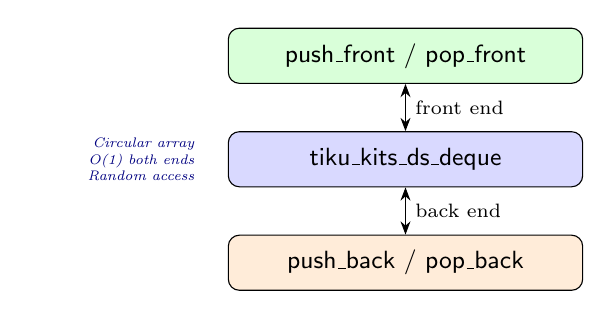
\begin{tikzpicture}[
    >=Stealth, node distance=0.5cm
  ]
  \node[draw, rounded corners, minimum height=0.7cm,
        text centered, font=\small\sffamily, fill=green!15,
        minimum width=4.5cm] (front) {push\_front / pop\_front};
  \node[draw, rounded corners, minimum height=0.7cm,
        text centered, font=\small\sffamily, fill=blue!15,
        minimum width=4.5cm, below=0.6cm of front] (dq)
    {tiku\_kits\_ds\_deque};
  \node[draw, rounded corners, minimum height=0.7cm,
        text centered, font=\small\sffamily, fill=orange!15,
        minimum width=4.5cm, below=0.6cm of dq] (back)
    {push\_back / pop\_back};
  \draw[<->] (front) -- node[right, font=\scriptsize] {front end} (dq);
  \draw[<->] (dq) -- node[right, font=\scriptsize] {back end} (back);

  \node[left=0.3cm of dq, font=\tiny\itshape, text=blue!50!black,
        text width=2cm, align=right] {Circular array\\O(1) both ends\\Random access};
\end{tikzpicture}
\end{center}

\vspace{0.5em}
\begin{alertblock}{Design Goal}
Provide a fixed-size double-ended queue with $O(1)$ push/pop at
\textbf{both ends}, $O(1)$ indexed access, \textbf{zero heap usage},
and clear bidirectional naming.
\end{alertblock}
\end{column}
\end{columns}
\end{frame}

% ===========================================================================
\section{Data Structure}
% ===========================================================================

\begin{frame}[fragile]{The \texttt{tiku\_kits\_ds\_deque} Structure}
\begin{columns}[T]
\begin{column}{0.48\textwidth}
\begin{lstlisting}[style=cstyle,
  title={ds/deque/tiku\_kits\_ds\_deque.h}]
#ifndef TIKU_KITS_DS_DEQUE_MAX_SIZE
#define TIKU_KITS_DS_DEQUE_MAX_SIZE 16
#endif

struct tiku_kits_ds_deque {
    tiku_kits_ds_elem_t
        data[TIKU_KITS_DS_DEQUE_MAX_SIZE];
    uint16_t head;      /* front index   */
    uint16_t tail;      /* back index    */
    uint16_t count;     /* valid elements*/
    uint16_t capacity;  /* user limit    */
};
\end{lstlisting}

\vspace{0.3em}
\textbf{Memory footprint:}\\
$16 \times 4 + 4 \times 2 = 72$ bytes (default).\\
All statically allocated --- no heap.
\end{column}

\begin{column}{0.48\textwidth}
\textbf{Circular array with two directions:}
\begin{center}
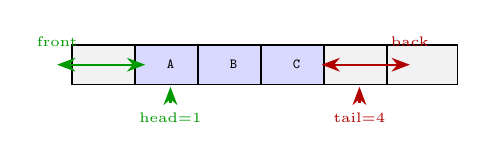
\begin{tikzpicture}[>=Stealth, scale=0.8]
  % Deque slots (horizontal)
  \foreach \i/\v in {0/{}, 1/A, 2/B, 3/C, 4/{}, 5/{}} {
    \pgfmathsetmacro{\fillcol}{\i > 0 && \i < 4 ? "blue!15" : "gray!10"}
    \node[draw, minimum width=0.9cm, minimum height=0.5cm,
          fill=\fillcol, font=\tiny\ttfamily] (s\i) at (\i*1.0, 0) {\v};
  }

  % Head and tail markers
  \draw[->, thick, green!60!black] (1*1.0, -0.6) -- (1*1.0, -0.35)
    node[below=0.2cm, font=\tiny] {head=1};
  \draw[->, thick, red!70!black] (4*1.0, -0.6) -- (4*1.0, -0.35)
    node[below=0.2cm, font=\tiny] {tail=4};

  % Arrows for both ends
  \draw[<->, thick, green!60!black] (-0.8, 0) -- (0.6, 0)
    node[above=0.1cm, font=\tiny, pos=0] {front};
  \draw[<->, thick, red!70!black] (3.4*1.0, 0) -- (4.8*1.0, 0)
    node[above=0.1cm, font=\tiny, pos=1] {back};
\end{tikzpicture}
\end{center}

\vspace{0.5em}
\begin{block}{Key Properties}
\begin{itemize}
  \item \texttt{head}: index of front element
  \item \texttt{tail}: index past the back element
  \item \texttt{count}: distinguishes full from empty
  \item Push front decrements head (wraps); push back increments tail (wraps)
\end{itemize}
\end{block}
\end{column}
\end{columns}
\end{frame}

% ===========================================================================
\section{Return Codes}
% ===========================================================================

\begin{frame}[fragile]{Shared Return Codes}
\begin{columns}[T]
\begin{column}{0.48\textwidth}
\begin{lstlisting}[style=cstyle,
  title={ds/tiku\_kits\_ds.h (shared)}]
typedef int32_t tiku_kits_ds_elem_t;

#define TIKU_KITS_DS_OK          0
#define TIKU_KITS_DS_ERR_NULL   -1
#define TIKU_KITS_DS_ERR_FULL   -2
#define TIKU_KITS_DS_ERR_EMPTY  -3
#define TIKU_KITS_DS_ERR_PARAM  -4
#define TIKU_KITS_DS_ERR_NOTFOUND -5
#define TIKU_KITS_DS_ERR_BOUNDS -6
\end{lstlisting}
\end{column}

\begin{column}{0.48\textwidth}
\begin{block}{Used by All DS Modules}
\begin{itemize}
  \item \texttt{ERR\_NULL} --- NULL pointer argument
  \item \texttt{ERR\_FULL} --- push when deque is at capacity
  \item \texttt{ERR\_EMPTY} --- pop/peek when deque is empty
  \item \texttt{ERR\_PARAM} --- invalid capacity at init
  \item \texttt{ERR\_BOUNDS} --- \texttt{get()} index out of range
\end{itemize}
\end{block}

\vspace{0.3em}
\begin{alertblock}{Deque-Specific}
The deque uses \texttt{ERR\_BOUNDS} for the indexed
\texttt{get()} operation --- an error code not needed by
simpler structures like stack or queue.
\end{alertblock}
\end{column}
\end{columns}
\end{frame}

% ===========================================================================
\section{API Reference}
% ===========================================================================

\begin{frame}[fragile]{Complete API}
\begin{table}
\centering
\small
\begin{tabular}{@{}lp{8cm}@{}}
\toprule
\textbf{Function} & \textbf{Description} \\
\midrule
\texttt{\_deque\_init(dq, cap)}
  & Initialize with capacity $1 \ldots$ \texttt{MAX\_SIZE}; zeros data \\
\texttt{\_deque\_push\_front(dq, val)}
  & Insert at front; decrement head with wrap \\
\texttt{\_deque\_push\_back(dq, val)}
  & Insert at back; increment tail with wrap \\
\texttt{\_deque\_pop\_front(dq, \&val)}
  & Remove from front; increment head with wrap \\
\texttt{\_deque\_pop\_back(dq, \&val)}
  & Remove from back; decrement tail with wrap \\
\texttt{\_deque\_peek\_front(dq, \&val)}
  & Read front element without removing \\
\texttt{\_deque\_peek\_back(dq, \&val)}
  & Read back element without removing \\
\midrule
\texttt{\_deque\_get(dq, idx, \&val)}
  & Read element at logical index; returns \texttt{ERR\_BOUNDS} \\
\texttt{\_deque\_count(dq)}
  & Return current number of elements \\
\texttt{\_deque\_full(dq)}
  & Return 1 if count $=$ capacity \\
\texttt{\_deque\_empty(dq)}
  & Return 1 if count $= 0$ \\
\texttt{\_deque\_clear(dq)}
  & Reset head, tail, count to 0 \\
\bottomrule
\end{tabular}
\end{table}

\vspace{0.3em}
{\scriptsize All functions are prefixed with \texttt{tiku\_kits\_ds}.
Every function validates pointer arguments and returns \texttt{ERR\_NULL} on failure.}
\end{frame}

% ===========================================================================
\section{Code Examples}
% ===========================================================================

\begin{frame}[fragile]{Example 1: Sliding Window Maximum}
\begin{lstlisting}[style=cstyle,
  title={Maintain the maximum over the last W sensor readings}]
#include "tikukits/ds/deque/tiku_kits_ds_deque.h"

#define WINDOW_SIZE 8

static struct tiku_kits_ds_deque idx_dq;   /* stores indices */
static int32_t readings[256];
static uint16_t n = 0;

void sliding_max_init(void) {
    tiku_kits_ds_deque_init(&idx_dq, WINDOW_SIZE);
}

/* Call once per new reading; returns the current window maximum */
int32_t sliding_max_update(int32_t value) {
    tiku_kits_ds_elem_t back_idx, front_idx;
    readings[n] = value;

    /* Remove indices of smaller elements from back */
    while (!tiku_kits_ds_deque_empty(&idx_dq)) {
        tiku_kits_ds_deque_peek_back(&idx_dq, &back_idx);
        if (readings[back_idx] <= value)
            tiku_kits_ds_deque_pop_back(&idx_dq, &back_idx);
        else break;
    }
    tiku_kits_ds_deque_push_back(&idx_dq, (int32_t)n);

    /* Remove expired indices from front */
    tiku_kits_ds_deque_peek_front(&idx_dq, &front_idx);
    if ((uint16_t)front_idx + WINDOW_SIZE <= n)
        tiku_kits_ds_deque_pop_front(&idx_dq, &front_idx);

    tiku_kits_ds_deque_peek_front(&idx_dq, &front_idx);
    n++;
    return readings[front_idx];  /* current window max */
}
\end{lstlisting}
\end{frame}

% ---------------------------------------------------------------------------
\begin{frame}[fragile]{Example 2: Priority Task Buffer}
\begin{columns}[T]
\begin{column}{0.48\textwidth}
\begin{lstlisting}[style=cstyle,
  title={Urgent tasks go to front, normal to back}]
#include "tiku_kits_ds_deque.h"

#define TASK_NORMAL  0
#define TASK_URGENT  1

static struct tiku_kits_ds_deque task_dq;

void task_buffer_init(void) {
    tiku_kits_ds_deque_init(&task_dq, 16);
}

/* Submit a task with priority */
int task_submit(int32_t task_id,
                int priority)
{
    if (priority == TASK_URGENT)
        return
          tiku_kits_ds_deque_push_front(
            &task_dq, task_id);
    else
        return
          tiku_kits_ds_deque_push_back(
            &task_dq, task_id);
}

/* Always dispatch from front */
int task_dispatch(int32_t *task_id) {
    return tiku_kits_ds_deque_pop_front(
        &task_dq, task_id);
}
\end{lstlisting}
\end{column}

\begin{column}{0.48\textwidth}
\begin{center}
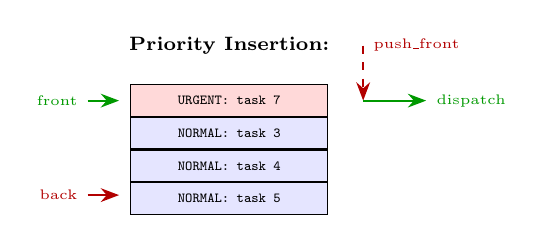
\begin{tikzpicture}[>=Stealth, node distance=0.15cm]
  \node[font=\scriptsize\bfseries] at (1.5, 3.5) {Priority Insertion:};

  % Deque visualization
  \node[draw, minimum width=2.5cm, minimum height=0.4cm,
        fill=red!15, font=\tiny\ttfamily] (u1) at (1.5, 2.8) {URGENT: task 7};
  \node[draw, minimum width=2.5cm, minimum height=0.4cm,
        fill=blue!10, font=\tiny\ttfamily, below=0cm of u1] (n1) {NORMAL: task 3};
  \node[draw, minimum width=2.5cm, minimum height=0.4cm,
        fill=blue!10, font=\tiny\ttfamily, below=0cm of n1] (n2) {NORMAL: task 4};
  \node[draw, minimum width=2.5cm, minimum height=0.4cm,
        fill=blue!10, font=\tiny\ttfamily, below=0cm of n2] (n3) {NORMAL: task 5};

  % Front/back labels
  \draw[->, thick, green!60!black] (-0.3, 2.8) -- (0.1, 2.8)
    node[left=0.4cm, font=\tiny] {front};
  \draw[->, thick, red!70!black] (-0.3, 1.6) -- (0.1, 1.6)
    node[left=0.4cm, font=\tiny] {back};

  % Arrow showing urgent push
  \draw[->, thick, red!70!black, dashed] (3.2, 3.5) -- (3.2, 2.8)
    node[right, font=\tiny, pos=0] {push\_front};

  % Dispatch arrow
  \draw[->, thick, green!60!black] (3.2, 2.8) -- (4.0, 2.8)
    node[right, font=\tiny] {dispatch};
\end{tikzpicture}
\end{center}

\vspace{0.5em}
\begin{block}{Pattern}
\begin{itemize}
  \item Normal tasks enqueue at back (FIFO)
  \item Urgent tasks push to front (priority)
  \item Dispatcher always pops from front
  \item Urgent tasks are processed first
\end{itemize}
\end{block}

\begin{alertblock}{Simpler than a Priority Queue}
For two priority levels, a deque is lighter than a
full priority queue --- no heap operations.
\end{alertblock}
\end{column}
\end{columns}
\end{frame}

% ===========================================================================
\section{Embedded Use Cases}
% ===========================================================================

\begin{frame}[fragile]{Use Case: Sliding Window Max for Sensor Anomaly Detection}
\begin{columns}[T]
\begin{column}{0.52\textwidth}
\begin{lstlisting}[style=cstyle,
  title={Detect anomaly spikes in sensor stream}]
#include "tiku_kits_ds_deque.h"

#define WIN_SIZE    8
#define SPIKE_RATIO 3  /* 3x above window max */

static struct tiku_kits_ds_deque win_dq;
static int32_t samples[256];
static uint16_t idx = 0;

void anomaly_init(void) {
    tiku_kits_ds_deque_init(&win_dq,
                            WIN_SIZE);
}

int anomaly_check(int32_t reading) {
    tiku_kits_ds_elem_t front, back;
    samples[idx] = reading;

    /* Maintain decreasing deque */
    while (!tiku_kits_ds_deque_empty(
               &win_dq)) {
        tiku_kits_ds_deque_peek_back(
            &win_dq, &back);
        if (samples[back] <= reading)
            tiku_kits_ds_deque_pop_back(
                &win_dq, &back);
        else break;
    }
    tiku_kits_ds_deque_push_back(
        &win_dq, (int32_t)idx);

    /* Expire old indices */
    tiku_kits_ds_deque_peek_front(
        &win_dq, &front);
    if ((uint16_t)front + WIN_SIZE <= idx)
        tiku_kits_ds_deque_pop_front(
            &win_dq, &front);

    /* Check spike against window max */
    tiku_kits_ds_deque_peek_front(
        &win_dq, &front);
    idx++;
    int32_t win_max = samples[front];
    if (reading > win_max * SPIKE_RATIO)
        return 1;  /* anomaly! */
    return 0;
}
\end{lstlisting}
\end{column}

\begin{column}{0.44\textwidth}
\begin{center}
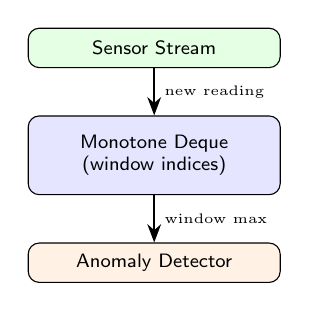
\begin{tikzpicture}[>=Stealth, node distance=0.4cm]
  \node[draw, rounded corners, fill=green!10,
        minimum width=3.2cm, minimum height=0.5cm,
        font=\scriptsize\sffamily] (sensor) {Sensor Stream};
  \node[draw, rounded corners, fill=blue!10,
        minimum width=3.2cm, minimum height=1.0cm,
        font=\scriptsize\sffamily, below=0.6cm of sensor,
        align=center] (dq)
    {Monotone Deque\\(window indices)};
  \node[draw, rounded corners, fill=orange!10,
        minimum width=3.2cm, minimum height=0.5cm,
        font=\scriptsize\sffamily, below=0.6cm of dq] (detect)
    {Anomaly Detector};

  \draw[->, thick] (sensor) -- node[right, font=\tiny] {new reading} (dq);
  \draw[->, thick] (dq) -- node[right, font=\tiny] {window max} (detect);
\end{tikzpicture}
\end{center}

\vspace{0.5em}
\begin{block}{Monotone Deque Technique}
\begin{itemize}
  \item Front always holds the window maximum index
  \item Back elements are removed if $\leq$ new value
  \item Expired indices removed from front
  \item $O(1)$ amortized per reading
\end{itemize}
\end{block}

\begin{alertblock}{Why Not Just Scan?}
A naive scan over $W$ elements costs $O(W)$ per reading.
The deque approach is $O(1)$ amortized --- critical
when $W$ is large or sample rates are high.
\end{alertblock}
\end{column}
\end{columns}
\end{frame}

% ===========================================================================
\section{Memory Layout}
% ===========================================================================

\begin{frame}{Memory Layout and Sizing}
\begin{columns}[T]
\begin{column}{0.48\textwidth}
\begin{center}
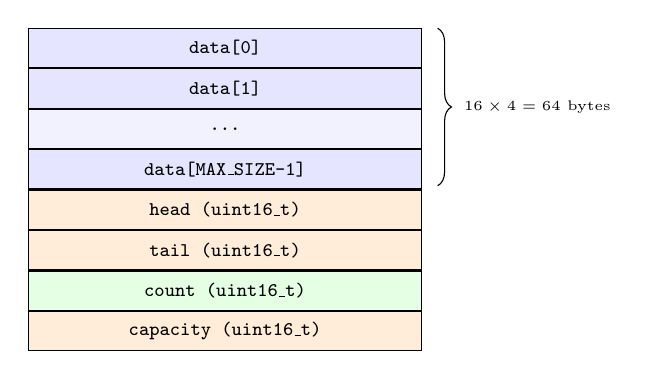
\begin{tikzpicture}[>=Stealth, node distance=0.0cm]
  \node[draw, minimum width=5cm, minimum height=0.5cm,
        fill=blue!10, font=\scriptsize\ttfamily] (d0) {data[0]};
  \node[draw, minimum width=5cm, minimum height=0.5cm,
        fill=blue!10, font=\scriptsize\ttfamily, below=0cm of d0] (d1) {data[1]};
  \node[draw, minimum width=5cm, minimum height=0.5cm,
        fill=blue!5, font=\scriptsize\ttfamily, below=0cm of d1] (d2) {...};
  \node[draw, minimum width=5cm, minimum height=0.5cm,
        fill=blue!10, font=\scriptsize\ttfamily, below=0cm of d2] (dn) {data[MAX\_SIZE-1]};
  \node[draw, minimum width=5cm, minimum height=0.5cm,
        fill=orange!15, font=\scriptsize\ttfamily, below=0cm of dn] (hd) {head (uint16\_t)};
  \node[draw, minimum width=5cm, minimum height=0.5cm,
        fill=orange!15, font=\scriptsize\ttfamily, below=0cm of hd] (tl) {tail (uint16\_t)};
  \node[draw, minimum width=5cm, minimum height=0.5cm,
        fill=green!10, font=\scriptsize\ttfamily, below=0cm of tl] (ct) {count (uint16\_t)};
  \node[draw, minimum width=5cm, minimum height=0.5cm,
        fill=orange!15, font=\scriptsize\ttfamily, below=0cm of ct] (cp) {capacity (uint16\_t)};

  \draw[decorate, decoration={brace, amplitude=5pt}]
    (2.7, 0.25) -- (2.7, -1.75)
    node[midway, right=6pt, font=\tiny] {$16 \times 4 = 64$ bytes};
\end{tikzpicture}
\end{center}
\end{column}

\begin{column}{0.48\textwidth}
\begin{block}{Size Formula}
\[
  \text{Total} = \texttt{MAX\_SIZE} \times \texttt{sizeof(elem\_t)} + 8
\]
\end{block}

\begin{table}
\centering
\scriptsize
\begin{tabular}{@{}rrr@{}}
\toprule
\textbf{MAX\_SIZE} & \textbf{elem\_t} & \textbf{Total (bytes)} \\
\midrule
4   & int32\_t & 24 \\
8   & int32\_t & 40 \\
16  & int32\_t & 72 \\
32  & int32\_t & 136 \\
8   & int16\_t & 24 \\
16  & int16\_t & 40 \\
\bottomrule
\end{tabular}
\end{table}

\vspace{0.3em}
\begin{alertblock}{Same Footprint as Queue}
The deque has the same memory layout as the queue
(head, tail, count, capacity) --- the extra functionality
comes from bidirectional index arithmetic, not extra storage.
\end{alertblock}
\end{column}
\end{columns}
\end{frame}

% ===========================================================================
\section{Complexity}
% ===========================================================================

\begin{frame}{Time Complexity}
\begin{table}
\centering
\begin{tabular}{@{}lcc@{}}
\toprule
\textbf{Operation} & \textbf{Best Case} & \textbf{Worst Case} \\
\midrule
\texttt{init}        & $O(n)$ & $O(n)$ \\
\texttt{push\_front} & $O(1)$ & $O(1)$ \\
\texttt{push\_back}  & $O(1)$ & $O(1)$ \\
\texttt{pop\_front}  & $O(1)$ & $O(1)$ \\
\texttt{pop\_back}   & $O(1)$ & $O(1)$ \\
\texttt{peek\_front} & $O(1)$ & $O(1)$ \\
\texttt{peek\_back}  & $O(1)$ & $O(1)$ \\
\texttt{get}         & $O(1)$ & $O(1)$ \\
\texttt{count}       & $O(1)$ & $O(1)$ \\
\texttt{clear}       & $O(1)$ & $O(1)$ \\
\bottomrule
\end{tabular}
\end{table}

\vspace{0.5em}
\begin{block}{All Core Operations Are $O(1)$}
\begin{itemize}
  \item Circular array with modulo wrap --- no element shifting
  \item \texttt{get(idx)} computes \texttt{(head + idx) \% capacity} --- direct access
  \item \texttt{init} is $O(n)$ due to \texttt{memset} zeroing the data array
  \item Constant, deterministic timing for every operation
  \item Safe for ISR contexts where timing must be predictable
\end{itemize}
\end{block}
\end{frame}

% ===========================================================================
\section{Test Suite}
% ===========================================================================

\begin{frame}{Test Cases Overview}
\begin{table}
\centering
\small
\begin{tabular}{@{}clp{7cm}@{}}
\toprule
\textbf{\#} & \textbf{Test Function} & \textbf{What It Verifies} \\
\midrule
1 & \texttt{test\_kits\_ds\_deque\_init}
  & Initialization, capacity bounds, empty/full state \\
2 & \texttt{test\_kits\_ds\_deque\_push\_pop\_front}
  & Push/pop at front, LIFO order from front \\
3 & \texttt{test\_kits\_ds\_deque\_push\_pop\_back}
  & Push/pop at back, LIFO order from back \\
4 & \texttt{test\_kits\_ds\_deque\_fifo\_order}
  & Push back, pop front returns FIFO order \\
5 & \texttt{test\_kits\_ds\_deque\_peek\_front\_back}
  & Peek both ends without removing \\
6 & \texttt{test\_kits\_ds\_deque\_get\_indexed}
  & Logical index access, bounds check \\
7 & \texttt{test\_kits\_ds\_deque\_full\_empty}
  & Full/empty flags, push-when-full error \\
8 & \texttt{test\_kits\_ds\_deque\_wraparound}
  & Head and tail wrap in both directions \\
9 & \texttt{test\_kits\_ds\_deque\_clear\_reset}
  & Clear resets state, operations after clear \\
10 & \texttt{test\_kits\_ds\_deque\_null\_inputs}
   & All functions reject NULL with ERR\_NULL \\
\bottomrule
\end{tabular}
\end{table}
\end{frame}

% ===========================================================================
\section{Summary}
% ===========================================================================

\begin{frame}{Summary}
\begin{columns}[T]
\begin{column}{0.48\textwidth}
\begin{block}{What We Built}
\begin{itemize}
  \item Fixed-capacity double-ended queue
  \item 12 API functions: init, push/pop/peek front and back, get, count, full, empty, clear
  \item Circular-array based $O(1)$ operations at both ends
  \item $O(1)$ random access via logical index
  \item Zero heap usage --- fully static
\end{itemize}
\end{block}

\begin{block}{Key Design Choices}
\begin{itemize}
  \item Bidirectional naming: push\_front/push\_back
  \item Count field for full/empty detection
  \item Default capacity 16
  \item \texttt{get()} provides indexed read access
  \item \texttt{empty(NULL)} returns 1 (safe default)
\end{itemize}
\end{block}
\end{column}

\begin{column}{0.48\textwidth}
\begin{block}{Use Cases}
\begin{itemize}
  \item Sliding window min/max algorithms
  \item Priority task buffers (urgent-to-front)
  \item Bidirectional stream processing
  \item Work-stealing schedulers
  \item Bounded undo history with FIFO eviction
\end{itemize}
\end{block}

\begin{block}{Files}
\scriptsize
\begin{tabular}{@{}lp{4.5cm}@{}}
Common: & \texttt{ds/tiku\_kits\_ds.h} \\
Header: & \texttt{ds/deque/tiku\_kits\_ds\_deque.h} \\
Source: & \texttt{ds/deque/tiku\_kits\_ds\_deque.c} \\
Tests:  & \texttt{tests/ds/test\_kits\_ds\_deque.c} \\
\end{tabular}
\end{block}
\end{column}
\end{columns}
\end{frame}

% ---------------------------------------------------------------------------
\begin{frame}{Thank You}
\begin{center}
\Large\textbf{TikuKits DS: Deque}\\[0.5em]
\normalsize Double-Ended Queue for Embedded Systems\\[1.5em]

\begin{tabular}{rl}
  Repository: & \url{https://github.com/tikuos/tikuOS} \\
  License:    & Apache 2.0 \\
  Common:     & \texttt{tikukits/ds/tiku\_kits\_ds.h} \\
  Header:     & \texttt{tikukits/ds/deque/tiku\_kits\_ds\_deque.h} \\
  Source:     & \texttt{tikukits/ds/deque/tiku\_kits\_ds\_deque.c} \\
  Tests:      & \texttt{tikukits/tests/ds/test\_kits\_ds\_deque.c} \\
\end{tabular}
\end{center}
\end{frame}

\end{document}
